%!TEX root = ../template.tex
%%%%%%%%%%%%%%%%%%%%%%%%%%%%%%%%%%%%%%%%%%%%%%%%%%%%%%%%%%%%%%%%%%%%%%
%% options.tex
%% NOVA thesis configuration file
%%
%% Processing of Class options
%%
%% Order and language for printing the abstracts depending on the language
%% These macros are just informative for now (it is hardcoded in the
%% 	novathesis.ldf file)… this must be fixed in the future!!
%%%%%%%%%%%%%%%%%%%%%%%%%%%%%%%%%%%%%%%%%%%%%%%%%%%%%%%%%%%%%%%%%%%%%%
%!TEX root = ../template.tex
%%%%%%%%%%%%%%%%%%%%%%%%%%%%%%%%%%%%%%%%%%%%%%%%%%%%%%%%%%%%%%%%%%%%%%
%% options.tex
%% NOVA thesis configuration file
%%
%% Processing of Class options
%%
%% Order and language for printing the abstracts depending on the language
%% These macros are just informative for now (it is hardcoded in the
%% 	novathesis.ldf file)… this must be fixed in the future!!
%%%%%%%%%%%%%%%%%%%%%%%%%%%%%%%%%%%%%%%%%%%%%%%%%%%%%%%%%%%%%%%%%%%%%%

\typeout{NT LOADING FILE options.tex}

%%%%%%%%%%%%%%%%%%%%%%%%%%%%%%%%%%%%%%%%%%%%%%%%%%%%%%%%%%%%%%%%%%%%%%%%
%% PROCESS KEY-VAL OPTIONS
%%%%%%%%%%%%%%%%%%%%%%%%%%%%%%%%%%%%%%%%%%%%%%%%%%%%%%%%%%%%%%%%%%%%%%%%%
\RequirePackage{options-nt}
\RequirePackage{xifthen}
\options{/@nt/.new family
  % languages
  , langsshort/.new list = {en, pt, fr, it, de, es}
  , langslong/.new list = {english, portuguese, french, italian, german, spanish}
  , langshorttolong/.new choice = {en=english, pt=portuguese, fr=french, it=italian, de=german, es=spanish}
  , maplang/.new cmd = {%
            \options{/@nt/langshorttolong = #1}%
            \option{/@nt/langshorttolong}%
  }  
  % %novathesis@opt@biblatex
  , biblatex/.new list
  , handler/school/.new cmd = {%
            \typeout{NT HANDLER SCHOOL ROUTINE [#1]}
            \ifoptiondefined{/@nt/cover/\option{/novathesis/school}/element}%
              {}% it as a reload… do nothing
              {% Load new school definitions
                \prependtographicspath{{NOVAthesisFiles/Schools/#1/Images/}}%
                \InputIfFileExists{NOVAthesisFiles/Schools/#1/defaults.ldf}%
                  {}%
                  {\PackageWarining{novathesis}%
                                   {Missing file “defaults.ldf” for #1}}%
              }%
  }
  , handler/media/.new cmd = {%
              \setulmarginsandblock%
                {\themargin(#1,top)}%
                {\themargin(#1,bottom)}%
                {*}%
              \setlrmarginsandblock%
                {\themargin(#1,left)}%
                {\themargin(#1,right)}%
                {*}%
              \checkandfixthelayout%
              \ifthenelse{\equal{\option{/novathesis/media}}{paper}}%
                {\options{/novathesis/linkscolor=black}}
                {}
  }
  , handler/chapstyle/.new cmd = {%
    \InputIfFileExists{NOVAthesisFiles/ChapStyles/#1.ldf}{}%
      {\PackageWarining{novathesis}{Invalid Chapter Style: #1}}
  }
  , handler/fontstyle/.new cmd = {%
    \InputIfFileExists{NOVAthesisFiles/FontStyles/#1.ldf}{}%
      {\PackageWarining{novathesis}{Invalid Font Style: #1}}
  }
  , ntfixspacing/.new toggle = false
}

\options{/novathesis/.new family
  , docdegree/.new choice = {phd, phdprop, phdplan, msc, mscplan, bsc},
  , school/.new choice = {{nova/fct}, {nova/fcsh}, {nova/ims}, {nova/ensp},
                          {ul/ist}, {ul/fc}, {ipl/isel}, {ips/ests}, {esep},
                          {iscte-iul/ista}, {consortium/msc-gt}}
  , docstatus/.new choice = {final, provisional, draft, working},
  , docstatus = final,
  , chapstyle/.new choice = {bianchi, bluebox, default, elegant, 
                             ell, hansen, ist, lyhne, madsen,
                            pedersen, section, southall, veelo,
                            vz34, vz43}
  , chapstyle=elegant        % set elegant as the default
  , fontstyle/.new choice = {kpfonts, bookman, erewhon, libertine, scholax,
                             calibri, kieranhealy}
  , fontstyle=kpfonts        % set kpfonts as the default
  , lang/.new style = {/novathesis/mainlang=#1,/novathesis/copyrightlang=#1,
                       /novathesis/coverlang=#1}
  , mainlang/.new choice = {en, pt, fr, it, de, es}
  , coverlang/.new choice = {en, pt, fr, it, de, es}
  , copyrightlang/.new choice = {en, pt, fr, it, de, es}
  , printcommittee/.new toggle = true
  , printcopyright/.new toggle = true
  , secondcover/.new toggle = false
  , aftercover/.new toggle = false
  , urlstyle/.new cmd = {%
            \edef\@nt@urlstyle{#1}\AfterPreamble{\urlstyle{\@nt@urlstyle}}%
  }
  , debugcover/.new toggle = false
  % , justcovers/.new toggle = false
  % , coverslist/.new list,
  , spine/.new toggle = false%
  , cdcover/.new toggle = false%
  , media/.new choice = {screen, paper}
  , linkscolor/.new cmd = {%
            \@ifpackageloaded{hyperref}%
              {\hypersetup{allcolors=#1,unicode}}%
              {\PassOptionsToPackage{allcolors=#1,unicode}{hyperref}}%
  }
}

\newcommand*{\ntsetup}[1]{%
  \ntgetkeyval{#1}\@nt@opt\@nt@value
  % \typeout{'NT SETUP = '[#1]~/~[\@nt@opt]~/~[\@nt@value]}
  \csuse{@nt@opt\@nt@opt @prehook}
  \options{/novathesis/\@nt@opt = {\@nt@value}}%
  % \typeout{'NT HANDLER = '/novathesis/handler/\@nt@opt}%
  \option{/@nt/handler/\@nt@opt}
  % \typeout{NT ->@nt@opt#1hook}
}

\newcommand*{\@nt@optschool@prehook}{%
}


\newcommand*{\ntbibsetup}[1]{\options{/@nt/biblatex/.push={#1}}}


% --------------------------------------------------------
% PROCESSING CLASS OPTIONS
\options@ProcessOptions{/novathesis}%


% --------------------------------------------------------
% FORCE SOME OPTIONS
\@AtEndClass{\options{/novathesis/printcommittee = false}}


% --------------------------------------------------------
% BABEL STUFF
\options@ProcessOptions{/novathesis}
\newcommand{\maplang}[1]{%
  \options{/@nt/maplang=#1}%
}

%
% % BABEL
\edef\nt@alllangs{}
\optionlistdo{/@nt/langsshort}{%
  \options{/@nt/langshorttolong=#1}%
  \ifoptionequal{/novathesis/mainlang}{#1}%
    {\edef\nt@alllangs{\nt@alllangs,main=\option{/@nt/langshorttolong}}}%
    {\edef\nt@alllangs{\nt@alllangs,\option{/@nt/langshorttolong}}}%
}
% \typeout{'NT PASSING TO BABEL = '\nt@alllangs}
\PassOptionsToPackage{\nt@alllangs}{babel}%

% --------------------------------------------------------
% Define DEFAULT VALUES for COVER and COPYRIGHT languages
\options{%
  /novathesis/coverlang = \option{/novathesis/mainlang}
  , /novathesis/copyrightlang = \option{/novathesis/mainlang}
  , /novathesis/linkscolor = RoyalBlue
}



% --------------------------------------------------------
% Pass the remaining options to memoir
\letoptionlist{/options/remaining}\nt@remaining
% \typeout{'NT PASSING TO MEMOIR='\nt@remaining}
\PassOptionsToClass{\nt@remaining}{memoir}



\AtEndDocument{%
  \iftoggle{/novathesis/spine}{%
    \InputIfFileExists{%
        NOVAthesisFiles/Schools/\option{/novathesis/school}/spine.tex%
    }%
      {}%
      {%!TEX root = ../template.tex
%%%%%%%%%%%%%%%%%%%%%%%%%%%%%%%%%%%%%%%%%%%%%%%%%%%%%%%%%%%%%%%%%%%%
%% spine.tex
%% NOVA thesis document template
%%
%% This work is licensed under the 
%% Creative Commons Attribution-NonCommercial 4.0 International License. 
%% To view a copy of this license, 
%% visit http://creativecommons.org/licenses/by-nc/4.0/.
%%
%% Authors / Contributors:
%%      - João Lourenço <joao.lourenco@fct.unl.pt>
%%      - Tomás Monteiro <monteiro.tomas@gmail.com>
%%%%%%%%%%%%%%%%%%%%%%%%%%%%%%%%%%%%%%%%%%%%%%%%%%%%%%%%%%%%%%%%%%%%%

\typeout{NT LOADING FILE spine.tex}


% Draw the book spine
% usable range: 145 to 425 pages, maximum characters for the title 140 and 22 for the author name
% usable range: 75 to 145 pages, maximum characters for the title 70 and 22 for the author name


\makeatletter

	\newlength{\@nt@spinewidth}%
	\setlength{\@nt@spinewidth}{0.5mm + 1mm * (\thelastsheet) / 20}% replace \thelastsheet by 1600 to get 80mm width folder label or any other value as long as the width is bigger than 50mm 

% Make a box with the logo
	\newbox{\@nt@spine@box@logo}%
	\newlength{\@nt@spine@box@logo@width}%
	\newlength{\@nt@spine@box@logo@height}%
	\newcommand{\@nt@spine@box@logoangle}{-90}%
	\newcommand{\make@spine@box@logo}[2]{%
	  \savebox{\@nt@spine@box@logo}{%
		\includegraphics%
		  [origin=c,angle=\@nt@spine@box@logoangle,height=0.95\@nt@spinewidth,#1]%
		  {#2}%
	  }%
    \ifdim\@nt@spinewidth > 22.2mm%
		  \savebox{\@nt@spine@box@logo}{%
		   \includegraphics%
		    [origin=c,angle=\@nt@spine@box@logoangle,height=22.2mm,#1]%
        {#2}
      }%
	  \fi%
	  \settowidth{\@nt@spine@box@logo@width}{\usebox{\@nt@spine@box@logo}}%
	  \settototalheight{\@nt@spine@box@logo@height}{\usebox{\@nt@spine@box@logo}}%
	}

% Make a box with the logo2
	\newbox{\@nt@spine@box@logotwo}%
	\newlength{\@nt@spine@box@logotwo@width}%
	\newlength{\@nt@spine@box@logotwo@height}%
	\newcommand{\@nt@spine@box@logotwoangle}{-90}%
	\newcommand{\make@spine@box@logotwo}[2]{%
	  \savebox{\@nt@spine@box@logotwo}{%
		\includegraphics%
		  [origin=c,angle=\@nt@spine@box@logotwoangle,height=0.95\@nt@spinewidth,#1]%
		  {#2}%
	  }%
    \ifdim\@nt@spinewidth > 22.2mm%
		  \savebox{\@nt@spine@box@logotwo}{%
       \includegraphics%
        [origin=c,angle=\@nt@spine@box@logotwoangle,height=22.2mm,#1]%
        {#2}
      }%
	  \fi%
	  \settowidth{\@nt@spine@box@logotwo@width}{\usebox{\@nt@spine@box@logotwo}}%
	  \settototalheight{\@nt@spine@box@logotwo@height}{\usebox{\@nt@spine@box@logotwo}}%
	}

% Make a box with the date
	\newbox{\@nt@spine@box@date}%
	\newlength{\@nt@spine@box@date@width}%
	\newlength{\@nt@spine@box@date@height}%
	\newcommand{\make@spine@box@date}{%
    % Print year into box
	  \savebox{\@nt@spine@box@date}{\thespine(year)}%
    % Get date box width and height
	  \settowidth{\@nt@spine@box@date@width}{\usebox{\@nt@spine@box@date}}%
	  \settototalheight{\@nt@spine@box@date@height}{\usebox{\@nt@spine@box@date}}%
    % Check if can print the date perpndicular to the book spine
	  \ifdim\@nt@spine@box@date@width < 0.9\@nt@spinewidth%
      \savebox{\@nt@spine@box@date}{%
		    \rotatebox[origin=c]{-90}{\usebox{\@nt@spine@box@date}}%
      }%
	  \fi%
    % Get date box width and height again 
	  \settowidth{\@nt@spine@box@date@width}{\usebox{\@nt@spine@box@date}}%
	  \settototalheight{\@nt@spine@box@date@height}{\usebox{\@nt@spine@box@date}}%
    % If larger than 95% spine width, resize to that dimension
	  \ifdim\@nt@spine@box@date@height > 0.9\@nt@spinewidth%
      \savebox{\@nt@spine@box@date}{%
		    \resizebox{!}{0.9\@nt@spinewidth}{\usebox{\@nt@spine@box@date}}%
      }%
	  \fi%
    % Get date box width and height yet again 
	  \settowidth{\@nt@spine@box@date@width}{\usebox{\@nt@spine@box@date}}%
	  \settototalheight{\@nt@spine@box@date@height}{\usebox{\@nt@spine@box@date}}%
	}




% Make a box with the title
	\newbox{\@nt@spine@box@title}%
	\newlength{\@nt@spine@box@title@width}%
	\newlength{\@nt@spine@box@title@height}%
	\newlength{\@nt@spine@box@middlewidth}%
	\newcommand{\make@spine@box@title}[1]{%
    % Find out how much is left for the title and author name
	  \setlength{\@nt@spine@box@middlewidth}{%
		  \dimexpr\paperheight-\@nt@spine@box@logo@height-\@nt@spine@box@date@height%
	  }%
    % Let's print the title in a single line and see how it looks
    \savebox{\@nt@spine@box@title}{\bfseries\thespine(title)}
    % Get title height
	  \settototalheight{\@nt@spine@box@title@height}{\usebox{\@nt@spine@box@title}}%
    % Check if height is larger than spine width, resize to spine width if necessary
    \ifdim\@nt@spine@box@title@height > 0.75\@nt@spinewidth%
     \savebox{\@nt@spine@box@title}{%
       \resizebox{!}{0.75\@nt@spinewidth}{\usebox{\@nt@spine@box@title}}%
      }%
    \fi
    % Get title width
	  \settowidth{\@nt@spine@box@title@width}{\usebox{\@nt@spine@box@title}}%
    % Check if width is larger than 70% of middlewidth, resize if necessary
    \ifdim\@nt@spine@box@title@width > 0.70\@nt@spine@box@middlewidth%
     \savebox{\@nt@spine@box@title}{%
       \resizebox{0.70\@nt@spine@box@middlewidth}{!}{\usebox{\@nt@spine@box@title}}%
      }%
    \fi
     \savebox{\@nt@spine@box@title}{%
       \setlength{\fboxsep}{0pt}
       \parbox{0.70\@nt@spine@box@middlewidth}{\centering\usebox{\@nt@spine@box@title}}%
       % \framebox[0.70\@nt@spine@box@middlewidth]{\usebox{\@nt@spine@box@title}}%
      }%
	  \settowidth{\@nt@spine@box@title@width}{\usebox{\@nt@spine@box@title}}%
	  \settototalheight{\@nt@spine@box@title@height}{\usebox{\@nt@spine@box@title}}%
	}


% Make a box with the author
	\newbox{\@nt@spine@box@author}%
	\newlength{\@nt@spine@box@author@width}%
	\newlength{\@nt@spine@box@author@height}%
	\newcommand{\make@spine@box@author}[1]{%
    % Find out how much is left for the author and author name
	  \setlength{\@nt@spine@box@middlewidth}{%
		  \dimexpr\paperheight-\@nt@spine@box@logo@height-\@nt@spine@box@date@height%
	  }%
    % Let's print the author in a single line and see how it looks
    \savebox{\@nt@spine@box@author}{\bfseries\thespine(author)}
    % Get author height
	  \settototalheight{\@nt@spine@box@author@height}{\usebox{\@nt@spine@box@author}}%
    % Check if height is larger than spine width, resize to spine width if necessary
    \ifdim\@nt@spine@box@author@height > 0.75\@nt@spinewidth%
     \savebox{\@nt@spine@box@author}{%
       \resizebox{!}{0.75\@nt@spinewidth}{\usebox{\@nt@spine@box@author}}%
      }%
    \fi
    % Get author width
	  \settowidth{\@nt@spine@box@author@width}{\usebox{\@nt@spine@box@author}}%
    % Check if width is larger than 70% of middlewidth, resize if necessary
    \ifdim\@nt@spine@box@author@width > 0.25\@nt@spine@box@middlewidth%
     \savebox{\@nt@spine@box@author}{%
       \resizebox{0.25\@nt@spine@box@middlewidth}{!}{\usebox{\@nt@spine@box@author}}%
      }%
    \fi
     \savebox{\@nt@spine@box@author}{%
       \setlength{\fboxsep}{0pt}
       \parbox{0.25\@nt@spine@box@middlewidth}{\centering\usebox{\@nt@spine@box@author}}%
       % \framebox[0.25\@nt@spine@box@middlewidth]{\usebox{\@nt@spine@box@author}}%
      }%
	  \settowidth{\@nt@spine@box@author@width}{\usebox{\@nt@spine@box@author}}%
	  \settototalheight{\@nt@spine@box@author@height}{\usebox{\@nt@spine@box@author}}%
	}

	
	
% Make the titleauthor group
	\newbox{\@nt@spine@box@titleauthor}%
	\newlength{\@nt@spine@box@titleauthor@width}%
	\newlength{\@nt@spine@box@titleauthor@height}%
	\newcommand{\make@spine@box@titleauthor}{%
	  \make@spine@box@title{0.8}%
	  \make@spine@box@author{0.8}%
	  \savebox{\@nt@spine@box@titleauthor}{%
		\parbox{0.8\@nt@spine@box@middlewidth}{%
		  % \vfill%
		  \usebox{\@nt@spine@box@title}%
		  \vfill%
		  \usebox{\@nt@spine@box@author}%
		  % \vfill%
		}%
	  }%
	  \settowidth{\@nt@spine@box@titleauthor@width}%
		{\usebox{\@nt@spine@box@titleauthor}}%
	  \settototalheight{\@nt@spine@box@titleauthor@height}%
		{\usebox{\@nt@spine@box@titleauthor}}%
	  \ifdim\@nt@spine@box@titleauthor@height > 0.90\@nt@spinewidth%
		\make@spine@box@title{0.90}%
		\make@spine@box@author{0.35}%
		\savebox{\@nt@spine@box@titleauthor}{%
		  \usebox{\@nt@spine@box@title}%  
		 \qquad~\qquad~\quad%
		  \usebox{\@nt@spine@box@author}%
		}%
	  \fi%
	
	  \settowidth{\@nt@spine@box@titleauthor@width}%
		{\usebox{\@nt@spine@box@titleauthor}}%
	  \settototalheight{\@nt@spine@box@titleauthor@height}%
		{\usebox{\@nt@spine@box@titleauthor}}%
	  \ifdim\@nt@spine@box@titleauthor@height > 0.90\@nt@spinewidth%
		\savebox{\@nt@spine@box@titleauthor}{%
		  \resizebox{!}{0.90\@nt@spinewidth}{\usebox{\@nt@spine@box@titleauthor}}%
		}%
	  \fi%
	  \settowidth{\@nt@spine@box@titleauthor@width}%
		{\usebox{\@nt@spine@box@titleauthor}}%
	  \settototalheight{\@nt@spine@box@titleauthor@height}%
		{\usebox{\@nt@spine@box@titleauthor}}%
	}



% start drawing things

	\newcommand{\AtStockLowerCenter}[1]{%
	  \AtPageUpperLeft{% 
		\put(\LenToUnit{(\paperwidth-\@nt@spinewidth)/2},%
			 \LenToUnit{-\paperheight}){#1}%
	  }%
	}


	\newbox{\@nt@spine@box}%
	\newcommand{\ntprintspine}{%
	  \clearforchapter%
	  \thispagestyle{empty}%
	  \make@spine@box@logo{}{\thespine(logo)}%
	  \ifexists{spine}[logotwo]{%
		\make@spine@box@logotwo{}{\thespine(logotwo)}%
	  }
	  \make@spine@box@date%
	  \make@spine@box@titleauthor%
	  \savebox{\@nt@spine@box}{%
		\rotatebox{90}{%
      \setlength{\fboxsep}{0pt}
		  \framebox[\stockheight]{%
			~~\hfill
			\parbox[c][\@nt@spinewidth][c]{\@nt@spine@box@date@width}%
			  {\usebox{\@nt@spine@box@date}}%
			\ifexists{spine}[logotwo]{%
			  \parbox[c][\@nt@spinewidth][c]{\@nt@spine@box@logotwo@width}%
				{\hspace*{3mm}\usebox{\@nt@spine@box@logotwo}}%
			}
%	        \hfill%
%	        \parbox[c][\@nt@spinewidth][c]{\@nt@spine@box@titleauthor@width}%
%	          {\usebox{\@nt@spine@box@titleauthor}}%
			\hfill%
			\parbox[c][\@nt@spinewidth][c]{\@nt@spine@box@title@width}%
			  {\usebox{\@nt@spine@box@title}}%
			\hfill%
			\parbox[c][\@nt@spinewidth][c]{\@nt@spine@box@author@width}%
			  {\usebox{\@nt@spine@box@author}}%
			\hfill
			\parbox[c][\@nt@spinewidth][c]{\@nt@spine@box@logo@width}%
			  {\usebox{\@nt@spine@box@logo}}%
			\hfill~~
		  }%
		}%
	  }%
	  
	  \ifdim\@nt@spinewidth > 50mm%
	  \savebox{\@nt@spine@box}{%
		\rotatebox{90}{%
		  \framebox[0.8\stockheight]{%
			~
			\parbox[c][\@nt@spinewidth][c]{\@nt@spine@box@date@width}%
			  {\usebox{\@nt@spine@box@date}}%
			\ifexists{spine}[logotwo]{%
			  \parbox[c][\@nt@spinewidth][c]{\@nt@spine@box@logotwo@width}%
				{\hspace*{3mm}\usebox{\@nt@spine@box@logotwo}}%
			}
%	        \hfill%
%	        \parbox[c][\@nt@spinewidth][c]{\@nt@spine@box@titleauthor@width}%
%	          {\usebox{\@nt@spine@box@titleauthor}}%
			\hfill%
			\parbox[c][\@nt@spinewidth][c]{\@nt@spine@box@title@width}%
			  {\usebox{\@nt@spine@box@title}}%
			\hfill%
			\parbox[c][\@nt@spinewidth][c]{\@nt@spine@box@author@width}%
			  {\usebox{\@nt@spine@box@author}}%
			\qquad
			\parbox[c][\@nt@spinewidth][c]{\@nt@spine@box@logo@width}%
			  {\usebox{\@nt@spine@box@logo}}%
			~
		  }%
		}%
	  }%
	  \fi%
	  \AddToShipoutPictureFG*{%
      \AtStockLowerCenter{{\usebox{\@nt@spine@box}}}%
	  }%
	  ~% This space is important here so that the spine page is not empty anymore!
	  % \clearforchapter%
	}%

\makeatother
}%
    \ntprintspine%
  }{}%
  \iftoggle{/novathesis/cdcover}{%
    \InputIfFileExists{%
        NOVAthesisFiles/Schools/\option{/novathesis/school}/cdcover.tex%
    }%
      {}%
      {%!TEX root = ../template.tex
%%%%%%%%%%%%%%%%%%%%%%%%%%%%%%%%%%%%%%%%%%%%%%%%%%%%%%%%%%%%%%%%%%%%
%% cdcover.tex
%% NOVA thesis document template
%%
%% This work is licensed under the 
%% Creative Commons Attribution-NonCommercial 4.0 International License. 
%% To view a copy of this license, 
%% visit http://creativecommons.org/licenses/by-nc/4.0/.
%%
%% Authors / Contributors:
%%      - João Lourenço <joao.lourenco@fct.unl.pt>
%%      - Tomás Monteiro <monteiro.tomas@gmail.com>
%%
%% This CD cover is a refactoring of the pull request by Tomás Monteiro
%% to reuse the information already provided in the file “template.tex”
%%%%%%%%%%%%%%%%%%%%%%%%%%%%%%%%%%%%%%%%%%%%%%%%%%%%%%%%%%%%%%%%%%%%%

\typeout{NT LOADING FILE cdcover.tex}


% Draw the cdcover


%% Cover: 12.0cm x 12.0cm
%% Inlay: 15.0cm x 11.8cm
%% Inlay fold: 0,635cm + 13,73cm + 0,635cm

\typeout{NT LOADING FILE cdcolver.ldf}

\makeatletter

\prependtographicspath{{NOVAthesisFiles/Images/}}

\newsavebox{\cdcover@savebox}

\newcommand{\ntprintcdcover}{%
	\clearpage

	\thispagestyle{empty}
	\pagestyle{empty}
	
	\setstocksize{12cm}{12cm}
	\settrimmedsize{\stockheight}{\stockwidth}{*}
	\settrims{0pt}{0pt}
	\setlrmarginsandblock{*}{-5mm}{*}
	\setulmarginsandblock{0mm}{*}{*}
	% \setlength{\parskip}{0pt}
	\setheadfoot{0mm}{0mm}
	\setheaderspaces{*}{0mm}{*}
	\setmarginnotes{0mm}{0mm}{0mm}
	\checkandfixthelayout[fixed]

  \AddToShipoutPictureBG*{
\includegraphics[width=120mm]{cd-cover-std}}

	\savebox{\cdcover@savebox}{%
	\begin{minipage}[t][7.0cm]{9cm}
		
		% Author name
		% \raggedright
		% \raggedleft
		\centering
		\fontsize{12}{12}\selectfont
		\textbf{\theauthorname}
		\medskip

		% Academic qualifications
		\fontsize{9}{9}\selectfont
		\theauthordegree
		\vfill

		% Title of Dissertation
		\fontsize{12}{12}\selectfont
		\textbf{\thetitle}
		\vfill

		% Degree
		\fontsize{9}{9}\selectfont
		\thepresentationtext
		\vfill

		% Date
		\fontsize{9}{9}\selectfont
		\textbf{\thentdatemonth, \thentdateyear}	
		
		
	\end{minipage}
	}

	~\\[1.75cm]~\hspace*{1.7cm}
	\usebox{\cdcover@savebox}

}

\newcommand{\ntprintcdinlay}{%
	\clearpage

	\thispagestyle{empty}
	\pagestyle{empty}
	
	\setstocksize{11.8cm}{15cm}
	\settrimmedsize{\stockheight}{\stockwidth}{*}
	\settrims{0pt}{0pt}
	\setlrmarginsandblock{*}{0mm}{*}
	\setulmarginsandblock{0mm}{*}{*}
	% \setlength{\parskip}{0pt}
	\setheadfoot{0mm}{0mm}
	\setheaderspaces{*}{0mm}{*}
	\setmarginnotes{0mm}{0mm}{0mm}
	\checkandfixthelayout[fixed]

  \AddToShipoutPictureBG*{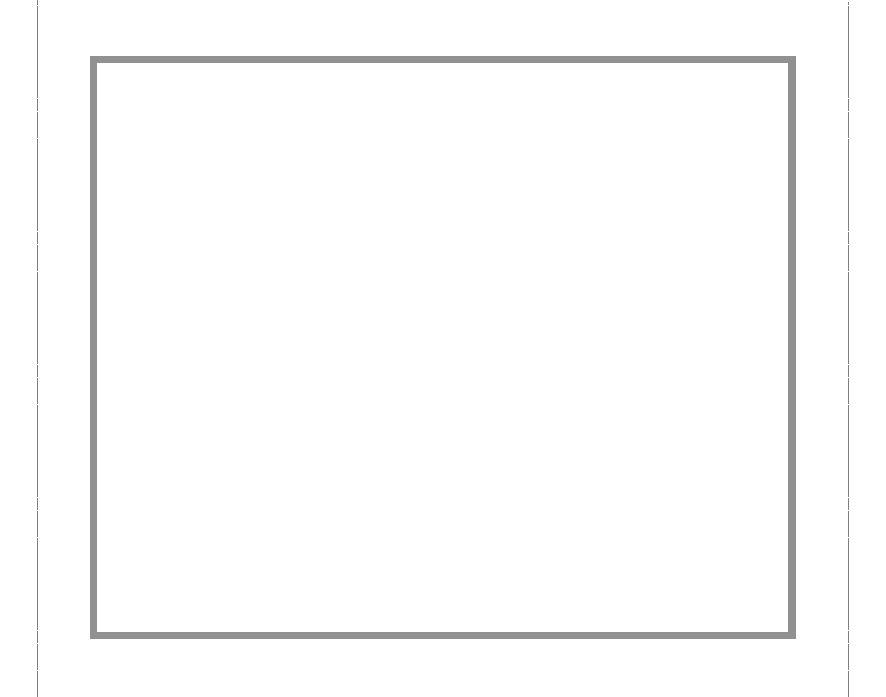
\includegraphics[width=150mm]{cd-inlay-std}}

	\savebox{\cdcover@savebox}{%
	\begin{minipage}[t][8cm]{11cm}
		
		% Author name
		% \raggedright
		% \raggedleft
		{
		\centering
		\vfill
		\fontsize{12}{12}\selectfont
		\textbf{\theauthorname}
		\medskip

		% Academic qualifications
		\fontsize{9}{9}\selectfont
		\theauthordegree
		\vfill

		% Title of Dissertation
		\fontsize{12}{12}\selectfont
		\textbf{\thetitle}
		\vfill

		% Degree
		\fontsize{9}{9}\selectfont
		\thepresentationtext
		\vfill

		% Date
		\fontsize{9}{9}\selectfont
		\textbf{\thentdatemonth, \thentdateyear}	
		\vfill

		}
		\fontsize{5}{7}\selectfont
		\thecopyrightstr
		
	\end{minipage}
	}
	
	\par

	\setlength{\fboxsep}{0pt}
	% ~\hspace*{1.8cm}
	~\\[0.75cm]~\hspace*{1.8cm}
	\usebox{\cdcover@savebox}
}

\makeatother
}%
    \ntprintcdcover%  
    \ntprintcdinlay%
  }{}%
}%
